\documentclass[a4paper,10pt]{article}
\usepackage{geometry}
\geometry{a4paper, portrait, margin=.8in}
\usepackage{amsmath,amsthm,amsfonts,amssymb,bbm,empheq}
\usepackage{paralist,graphics,epsfig,graphicx,epstopdf,mathrsfs}
\usepackage{float,color,ulem,comment,tabulary,cite,booktabs}
\usepackage{multirow,multicol}
\usepackage{epsf,epsfig,subfigure}
\setcounter{MaxMatrixCols}{30}
\usepackage[colorlinks=true]{hyperref}
\hypersetup{urlcolor=blue,linkcolor=black,citecolor=blue,colorlinks=true}
% \usepackage[notref,notcite]{showkeys}
\usepackage{mathpazo}
\usepackage[table,xcdraw]{xcolor}
\usepackage{cite}
\usepackage{svg}

\newcommand{\red}[1]{\textcolor{red}{#1}}
\title{VAE-CME}
\author{Xinyi Zhou}
\date{2023.6.23}

\begin{document}
\tableofcontents
\maketitle

\section{Birth Death Model}
Consider a simple non-Markovian system where molecules are produced at a rate $\rho$ and are removed from the system (degraded) after a fxed time delay $\tau$:
\begin{equation}\label{birth-death}
\emptyset\stackrel{\rho}\rightarrow N, N\stackrel{\tau}\Rightarrow\emptyset
\end{equation}
The training set is the distribution from $1 \times 10^4$ samples using the SSA.In the experiment, we assume $\rho=20$, $\tau=10$ and truncation $N=271$. 

Both encoder and decoder are multilayer perceptron with one hidden layer. The objective function is chosen as the sum of mean-squared-error and KL divergence. For the training we used the standard adaptive moment estimation algorithm (ADAM). The weight of mean-squared-error needs to be increased, and the learning rate needs to be decreased from approximately 0.25 to 0.01 during the training process. The fitting performance after training is shown in Fig. \ref{Birth Death Model Fitting}.

\begin{figure*}[h]
	\centering
	\includegraphics[width=0.6\textwidth]{Figs/Birth_Death_fitting.pdf}
	\caption{Birth Death Model Fitting}\label{Birth Death Model Fitting}  
\end{figure*}

\section{On Off Model}
We also consider On Off Model wherein the promoter switches between an active and inactive state, RNAP binding occurs only in the active state, which is followed by delayed degradation modelling the RNAP movement along the gene and its detachment; this can be described by the reaction scheme:
\begin{equation}\label{on-off}
	\begin{aligned}
	G^*\xrightarrow{k_{\text{on}}} G,
	G\xrightarrow{k_{\text{off}}}G^*,
	G\xrightarrow{\rho}G+N.
	\end{aligned}
\end{equation}
The same as Birth Death Model, The training set is the distribution from $1 \times 10^4$ samples using the SSA.In the experiment, we assume $k_{\text{on}}=1$, $k_{\text{off}}=1$, $\rho=20$, and truncation $N=45$.

The same objective function, optimizer, and adjustments to weights and learning rate are used for training as in the Birth Death Model. The fitting performance after training is shown in Fig. \ref{On Off Model fitting}. 

\begin{figure*}[h]
	\centering
	\includegraphics[width=0.6\textwidth]{Figs/On_Off_fitting.pdf}
	\caption{On Off Model fitting}\label{On Off Model fitting}  
\end{figure*}

\section{Bursty Model}

We consider Bursty Model, which is the same as Birth Death Model, except that the binding of RNAPs to the promoter occurs in bursts whose size $i$ is distributed according to the geometric distribution $b^i/(1 + b)^{i+1}$; this can be described by the reaction scheme:
\begin{equation}\label{bursty}
	\begin{aligned}
		&\emptyset\stackrel{\frac{\alpha b^i}{(1+b)^{i+1}}}\longrightarrow iN,i=1,2,3,...\\ &N\stackrel{\tau}\Rightarrow\emptyset
	\end{aligned}
\end{equation}
To achieve the best fitting performance, the analytical solution of the Bursty model's probability distribution (See SI in \cite{jiang2021neural}) is used as the training set. In the experiment, we assume $\alpha=0.0282$, $b=3.46$, $\tau=120$ and truncation $N=64$.

The same as before, we choose the sum of mean-squared-error and KL divergenc as the  objective  function, ADAM as the optimizer. The weight of mean-squared-error needs to be increased, and the learning rate needs to be decreased. The fitting performance after training is shown in Fig. \ref{Bursty Model Fitting}
\begin{figure*}[h]
	\centering
	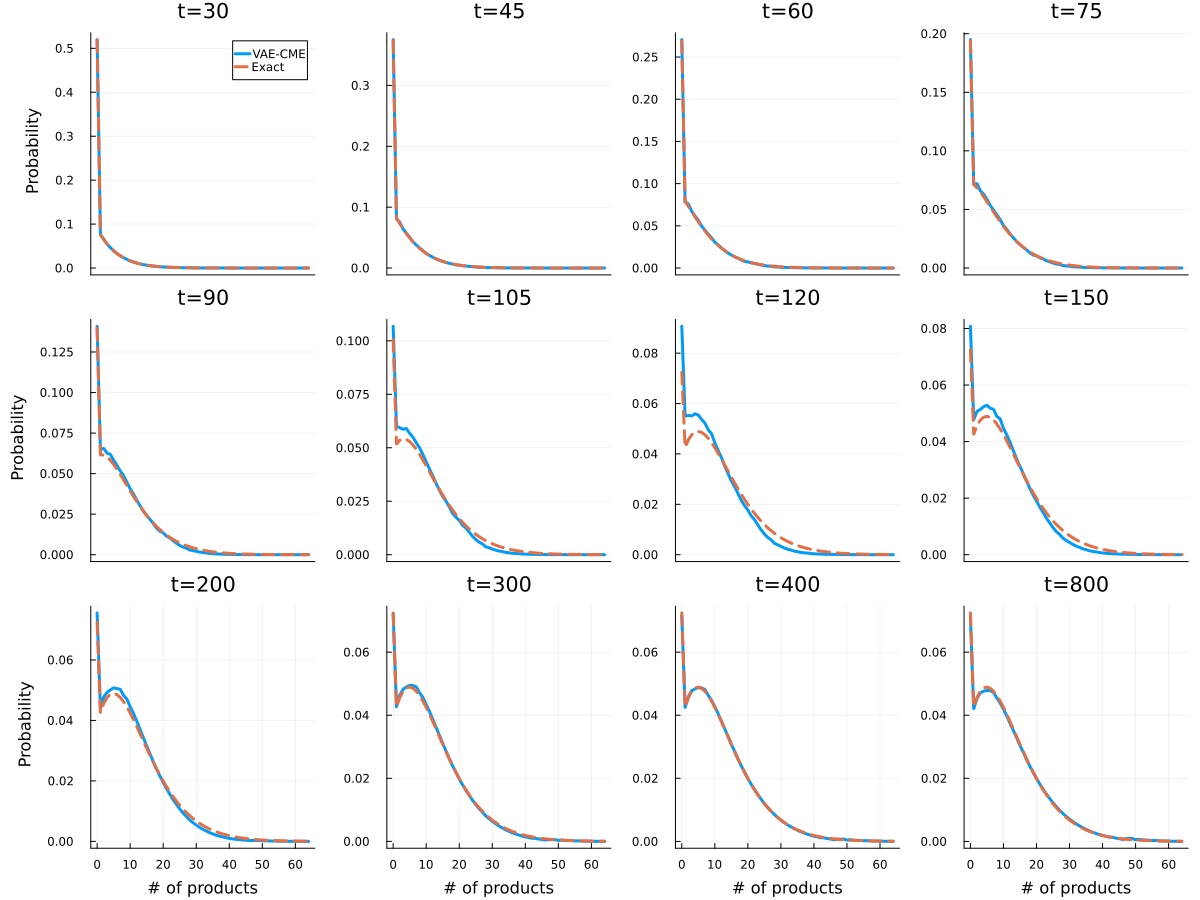
\includegraphics[width=0.6\textwidth]{Figs/Bursty_fitting.pdf}
	\caption{Bursty Model Fitting}\label{Bursty Model Fitting}  
\end{figure*}

\subsection{Control Mean of time delay $\tau$}
We have designed one encoder and two decoders. The two decoders are designed to reconstruct the probability distributions of $\tau=30$ and $\tau=120$, respectively. The two decoders share the same set of parameters. An additional node, which we call Attribute in this paper, is added to the input layer of the decoder (i.e., the latent space). For the decoder corresponding to $\tau=120$, the value of the additional node is set to 1. For the decoder corresponding to $\tau=30$, the value of the additional node is set to 0. The  objective  function  ischosen as the sum of mean-squared-error between the outputs of the two decoders and the probability distributions obtained for Bursty Model of $\tau=30$ and $\tau=120$ and KL divergence. To achieve the best fitting performance, we choose the analytical solution of the Bursty model’s probability distributions as the training set. The fitting performance after training is shown in Figs. \ref{Bursty_fitting_tau=30}-\ref{Bursty_fitting_tau=120}.
\begin{figure*}[h]
	\centering
	\includegraphics[width=0.6\textwidth]{Figs/Bursty_fitting_tau=30.pdf}
	\caption{Bursty Model Fitting $\tau=30$}\label{Bursty_fitting_tau=30}  
\end{figure*}
\begin{figure*}[h]
	\centering
	\includegraphics[width=0.6\textwidth]{Figs/Bursty_fitting_tau=120.pdf}
	\caption{Bursty Model Fitting $\tau=120$}\label{Bursty_fitting_tau=120}  
\end{figure*}
Inspired by the set of biases in the output layer, which is $r_n=\frac{n}{\tau}$\cite{jiang2021neural}, $n=1,...,N$, we found that there is a proportional relationship between the Attribute and $1/\tau$(See Fig. \ref{tau_Attribute}). Following this proportional relationship, it is possible to predict the probability distributions obtained by the Bursty Model for any elongation time $\tau$ between 30 and 120. The predicting performance is shown in Figs. \ref{Bursty_predicting_tau=40}-\ref{Bursty_predicting_tau=100}
\begin{figure*}[h]
	\centering
	\includegraphics[width=0.4\textwidth]{Figs/tau_Attribute.pdf}
	\caption{1/$\tau$ Attribute}\label{tau_Attribute}  
\end{figure*}
\begin{figure*}[h]
	\centering
	\includegraphics[width=0.6\textwidth]{Figs/Bursty_predicting_tau=40.pdf}
	\caption{Bursty Model Predicting $\tau=40$}\label{Bursty_predicting_tau=40}  
\end{figure*}
\begin{figure*}[h]
	\centering
	\includegraphics[width=0.6\textwidth]{Figs/Bursty_predicting_tau=60.pdf}
	\caption{Bursty Model Predicting $\tau=60$}\label{Bursty_predicting_tau=60}  
\end{figure*}
\begin{figure*}[h]
	\centering
	\includegraphics[width=0.6\textwidth]{Figs/Bursty_predicting_tau=100.pdf}
	\caption{Bursty Model Predicting $\tau=100$}\label{Bursty_predicting_tau=100}  
\end{figure*}
\subsection{Control Variance of time delay $\tau$}
When the elongation time $\tau$ is a random variable sampled from a distribution, VAE alse works very well. Here we assume $\tau$ follows a two-point distribution, it means that it can take only two discrete values,$\tau_1$ and $\tau_2$ with probabilities $p$ and $1-p$, respectively. In the experiment, we assume $\alpha=0.0282$, $b=3.46$, $p=0.6$. We obtain five sets of data by different values of $\tau$ (See Table. \ref{table of tau}). Note that the mean value of $\tau$ is 120 across these five sets of data.
\begin{table}[H]
	\centering
	  \scriptsize
	  \begin{tabular}{c|ccc}
		  \toprule
		  dataset & $\tau_1$ & $\tau_2$ & Variance \\
		  \cmidrule{1-4}
		  dataset \#1 & L/3   & L      & 4266 \\
		  dataset \#2 & 3L/10 & 1.05L  & 5400 \\
		  dataset \#3 & L/4   & 1.125L & 7350 \\
	      dataset \#4 & L/5   & 1.2L   & 9600 \\
	      dataset \#5 & L/6   & 1.25L  & 11266 \\
	  \bottomrule
	  \end{tabular}
	  \caption{Value of $\tau$, $L=200$}
	  \label{table of tau}
\end{table}
We use dataset \#1 and dataset \#5 as the training sets, and the remaining datasets will be used as the prediction sets. The same as before, the two decoders are designed to reconstruct the probability distributions of dataset \#1 and dataset \#5, the corresponding attribute values are 0 and 1, respectively. Figs \ref{Bursty_fitting_var=4266}-\ref{Bursty_fitting_var=11266} show the fitting performance of dataset \#1 and dataset \#5.
\begin{figure*}[h]
	\centering
	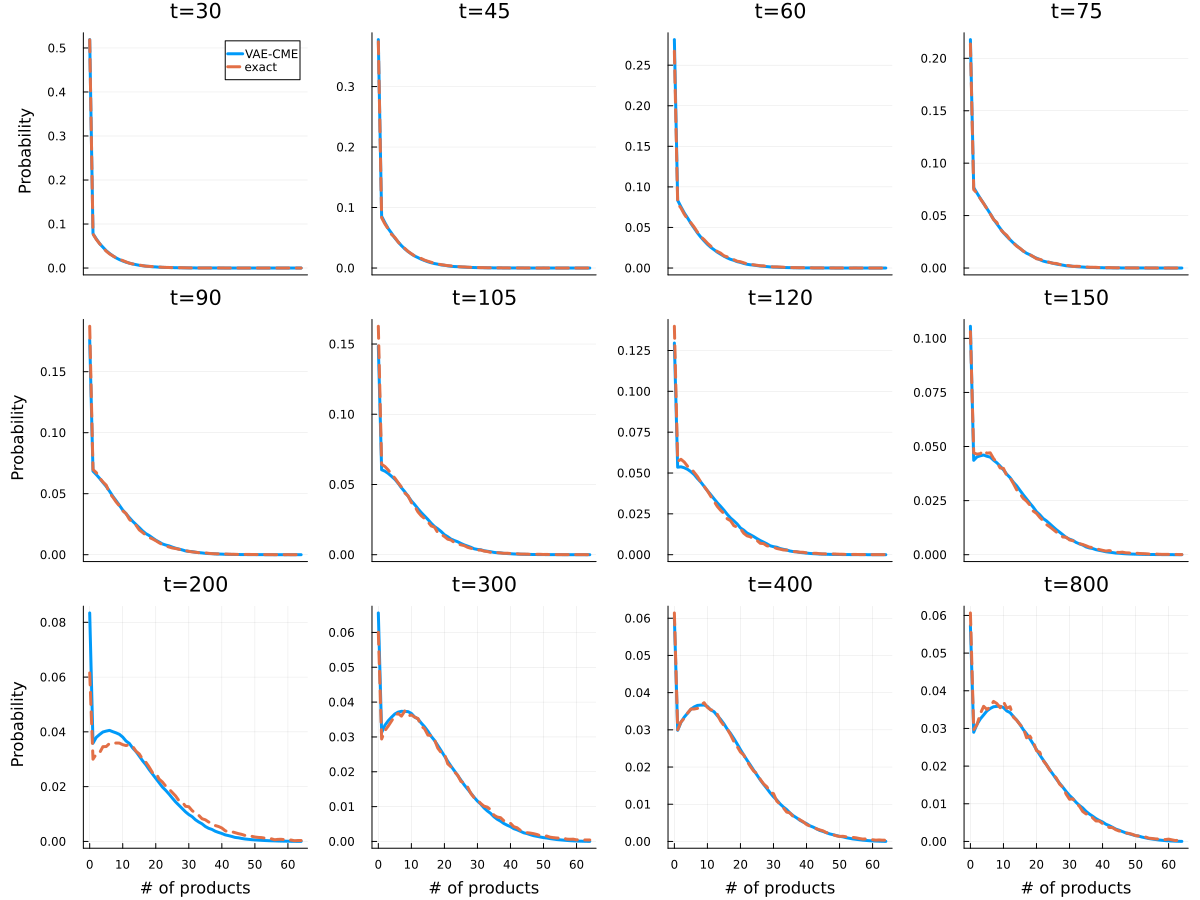
\includegraphics[width=0.6\textwidth]{Figs/fit_var=4266.pdf}
	\caption{Bursty Model Fitting Variance=4266}\label{Bursty_fitting_var=4266}  
\end{figure*}
\begin{figure*}[h]
	\centering
	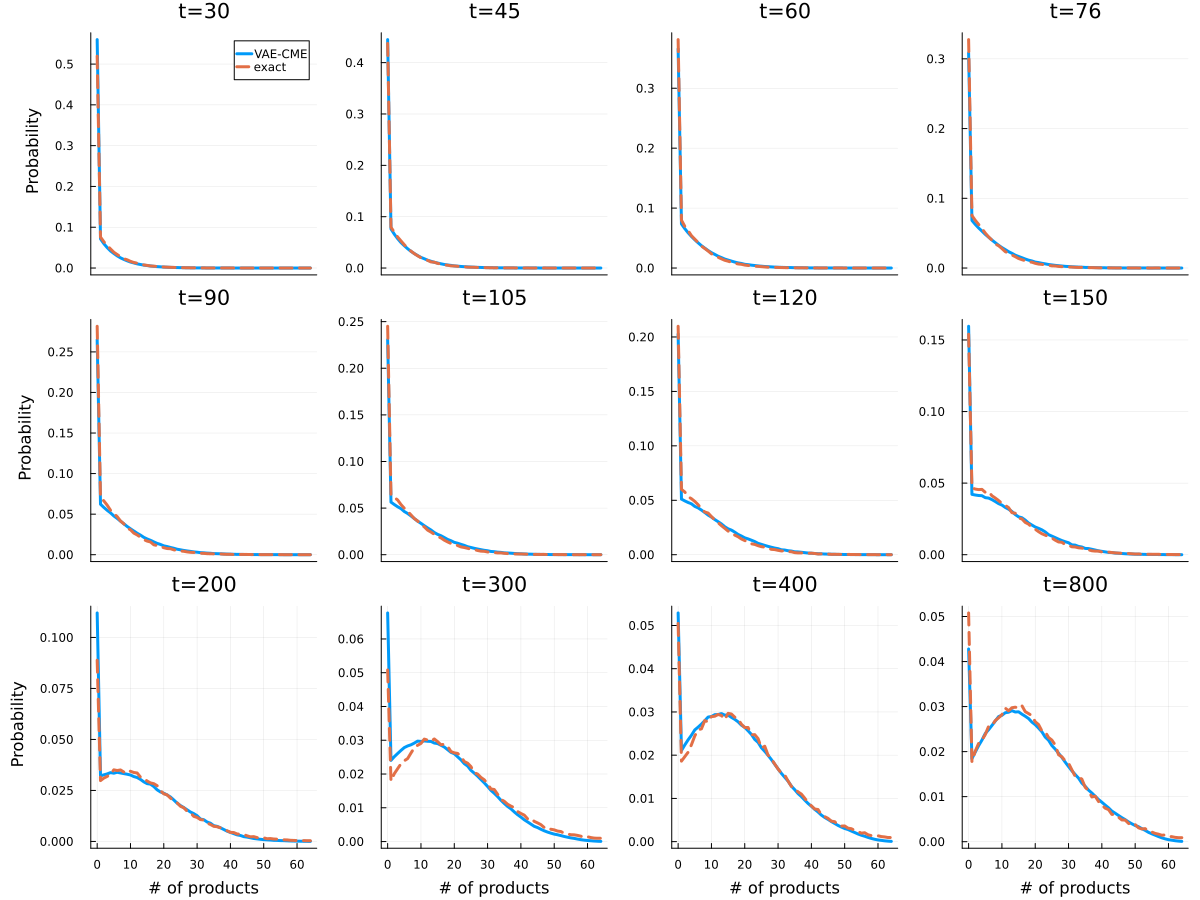
\includegraphics[width=0.6\textwidth]{Figs/fit_var=11266.pdf}
	\caption{Bursty Model Fitting Variance=11266}\label{Bursty_fitting_var=11266}  
\end{figure*}

We found that there is a proportional relationship between the Attribute and $T_1$ or $T_2$ (See Fig. \ref{T1orT2_Attribute}). Figs \ref{Bursty_predicting_var=5400}-\ref{Bursty_predicting_var=9600} show the predicting performance of the remaining datasets.
\begin{figure*}[h]
	\centering
	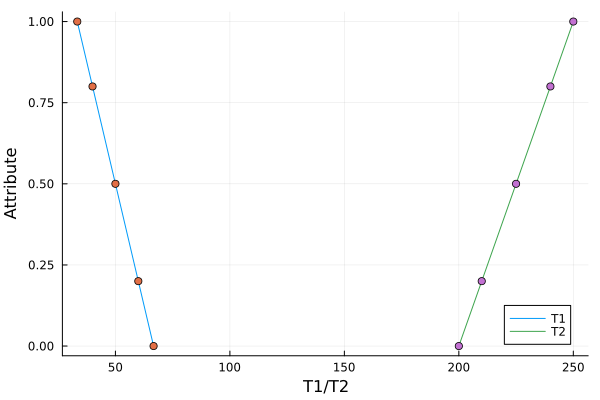
\includegraphics[width=0.4\textwidth]{Figs/T1orT2_Attribute.pdf}
	\caption{$\tau_1$ or $\tau_2$ Attribute}\label{T1orT2_Attribute}  
\end{figure*}
\begin{figure*}[h]
	\centering
	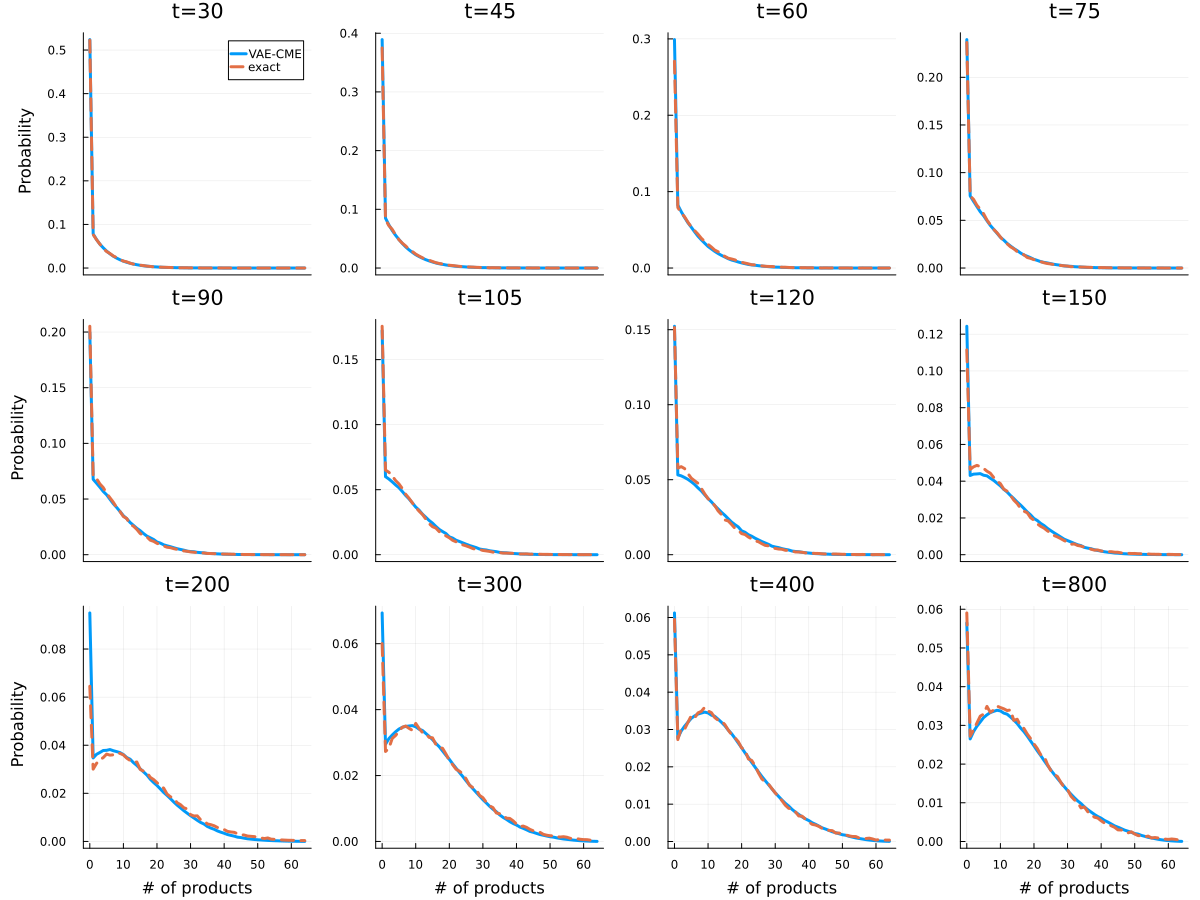
\includegraphics[width=0.6\textwidth]{Figs/predict_var=5400.pdf}
	\caption{Bursty Model Predicting Variance=5400}\label{Bursty_predicting_var=5400}  
\end{figure*}
\begin{figure*}[h]
	\centering
	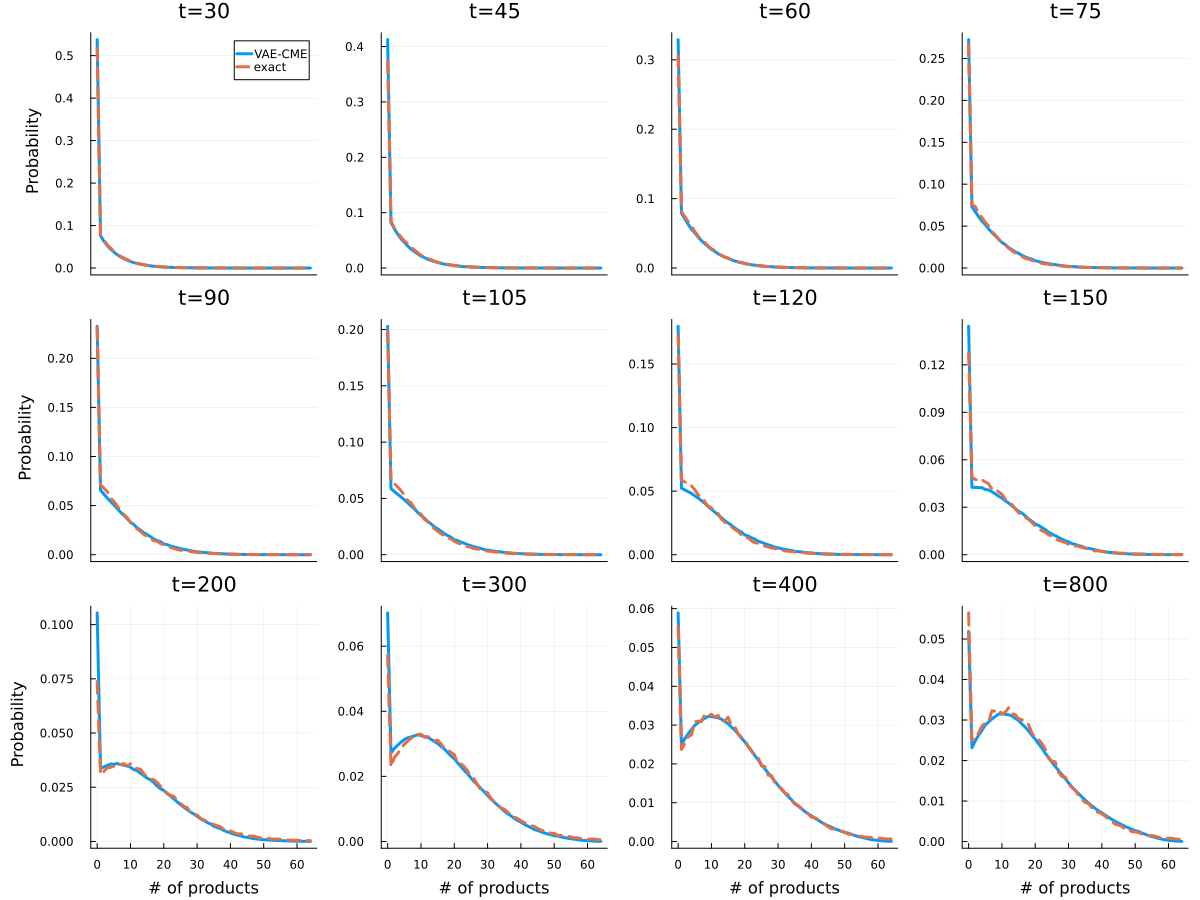
\includegraphics[width=0.6\textwidth]{Figs/predict_var=7350.pdf}
	\caption{Bursty Model Predicting Variance=7350}\label{Bursty_predicting_var=7350}  
\end{figure*}
\begin{figure*}[h]
	\centering
	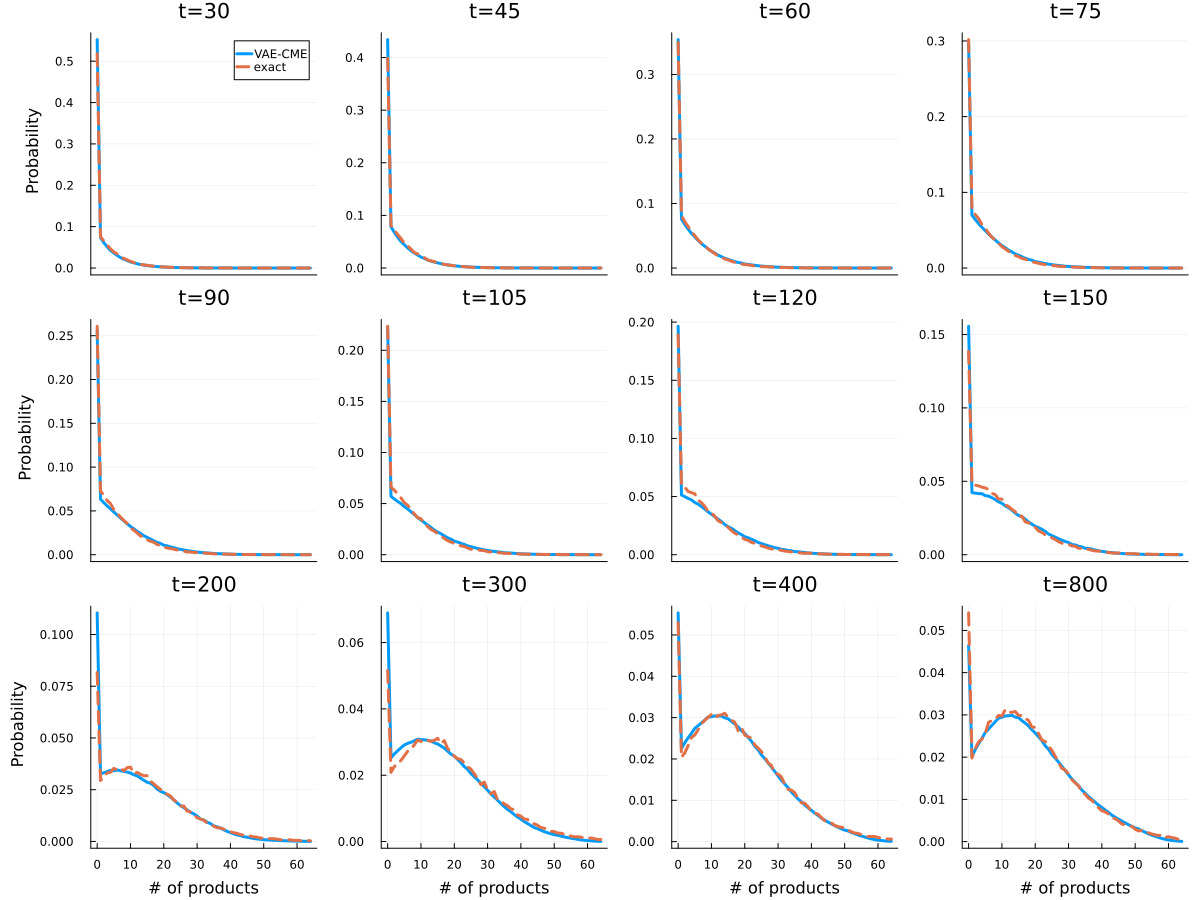
\includegraphics[width=0.6\textwidth]{Figs/predict_var=9600.pdf}
	\caption{Bursty Model Predicting Variance=9600}\label{Bursty_predicting_var=9600}  
\end{figure*}










\section{Oscillation Model}
Here we consider Oscillation Model, which is a simple genetic negative feedback loop whereby (i) a protein $X$ is transcribed by a promoter, (ii) subsequently after a fixed time delay $\tau$, $X$ turns (via some set of unspeci"ed biochemical processes) into a protein $Y$ and (iii) finally Y binds the promoter and reduces the rate of transcription of $X$. This can be described by the reaction scheme:
\begin{equation}\label{oscillation}
	\begin{aligned}
		\emptyset \xrightarrow{J_1(Y)} X,
		X\stackrel{\tau}\Rightarrow Y,
		Y\xrightarrow{J_2(Y)} \emptyset.
	\end{aligned}
\end{equation}

The function $J_1(Y)$ and $J_2(Y)$ is defined as follows:
\begin{equation}\label{oscillation}
	\begin{aligned}
	J_1(Y)=k_1S\frac{K^p_d}{K^p_d+Y^p},\\
	J_2(Y)=k_2E_T\frac{Y}{K_m+Y}.
	\end{aligned}
\end{equation}
In this example, we assume $k_1=k_2=S=E_T=K_d=K_m=1, p=2$ for simplicity. Unlike Models considered earlier, the delay master equation corresponding to this model has no known analytical solution. The training set is the distribution from $1 \times 10^4$ samples using the SSA. Moreover, we assume $\tau=10$ and truncation $N=26$.

We only use the simulated trajectories of mature protein Y to train the VAE. In other words, the data of protein $X$ is not required during training. However, an additional regularization term which is the first derivative of the probability distribution of protein $X$ obtained from the chemical master equation (CME), needs to be added to the objective function. Therefore, the final objective function of this experiment is the sum of mean-squared-error of protein $Y$, KL divergence and regularization term mentioned before. The fitting performance of protein $Y$ after training is shown in Fig. \ref{Oscillation_Y_fitting} and the predicting performance of protein $X$ is shown in Fig. \ref{Oscillation_X_predicting}.
\begin{figure*}[h]
	\centering
	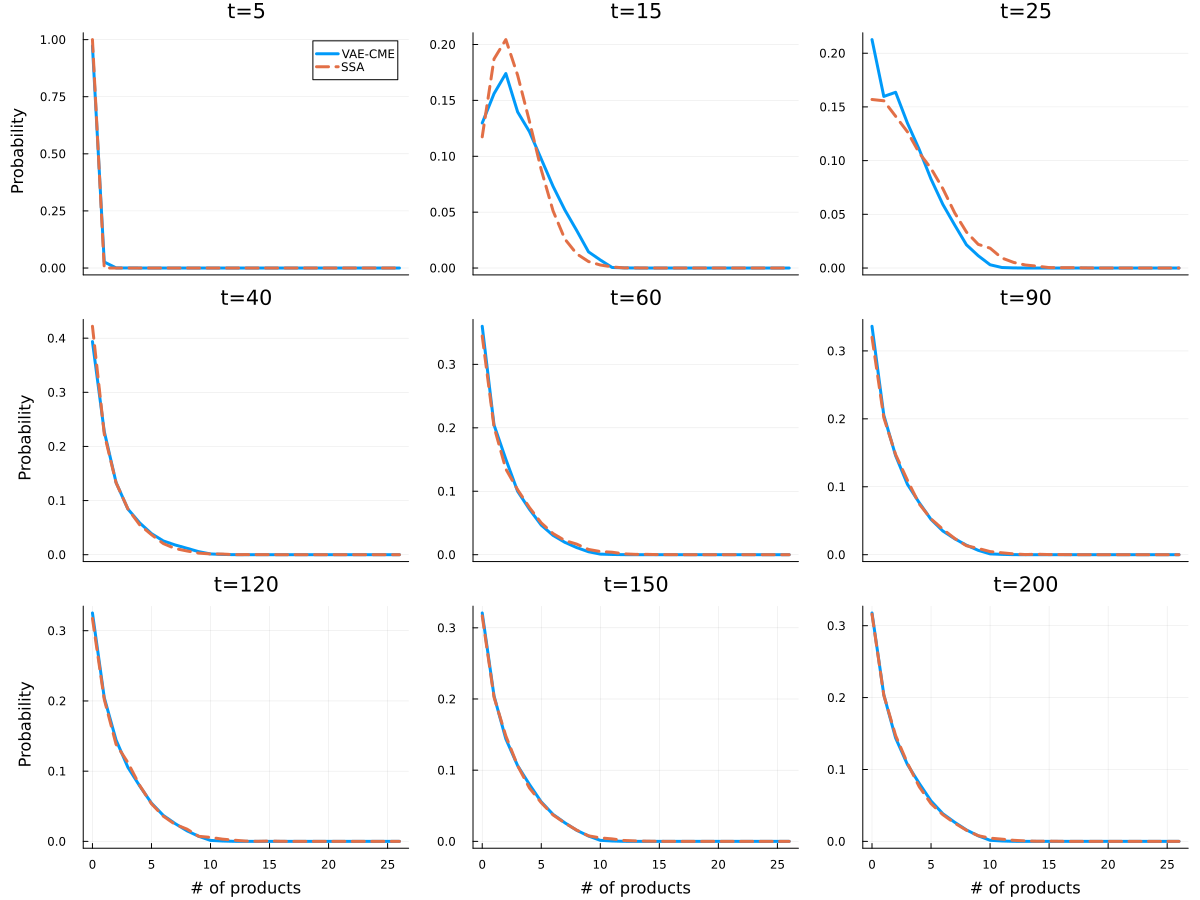
\includegraphics[width=0.6\textwidth]{Figs/Oscillation_Y_fitting.pdf}
	\caption{Oscillation Y fitting}\label{Oscillation_Y_fitting}  
\end{figure*}
\begin{figure*}[h]
	\centering
	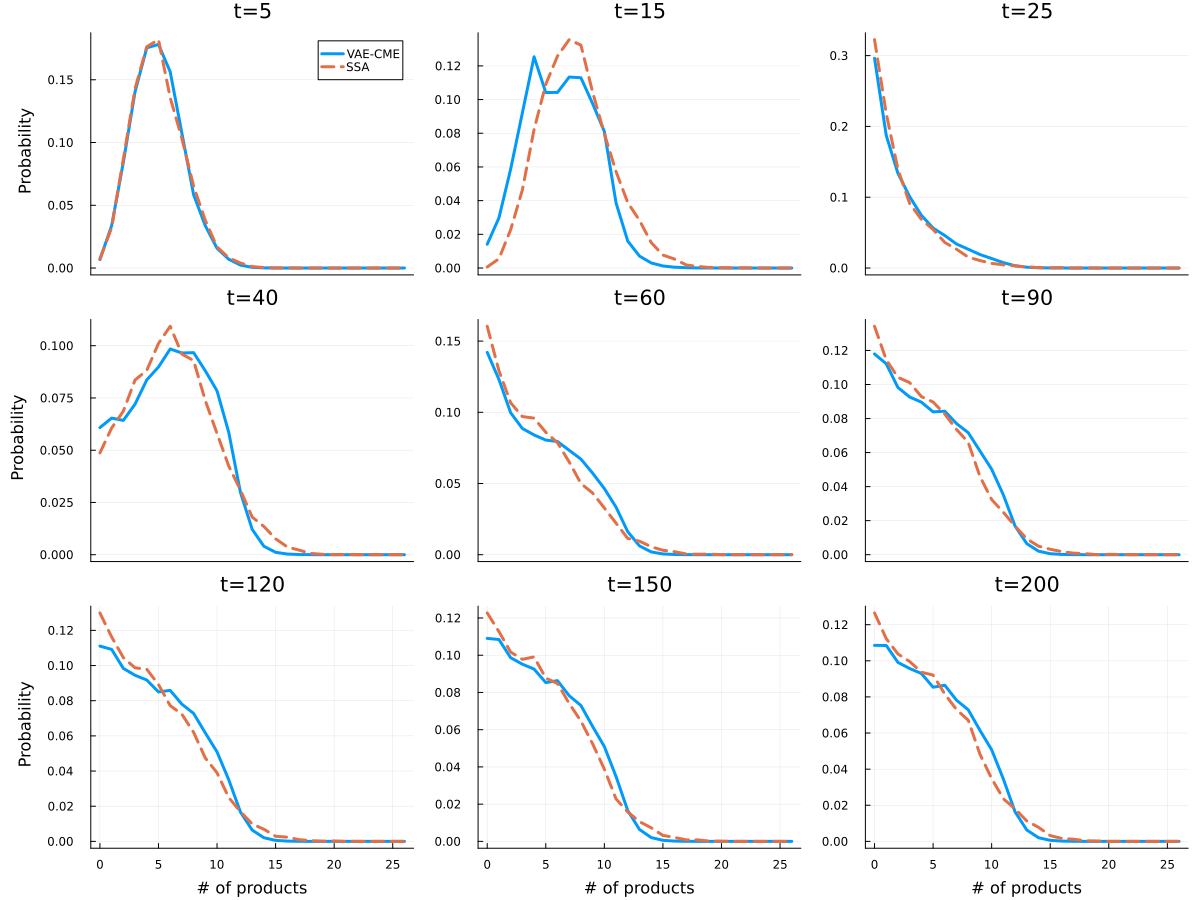
\includegraphics[width=0.6\textwidth]{Figs/Oscillation_X_predicting.pdf}
	\caption{Oscillation X predicting}\label{Oscillation_X_predicting}  
\end{figure*}
\subsection{Reducing sample size}
Due to the poor predicting performance of MLP\cite{jiang2021neural} on protein $X$ in the Oscillation model, we studied the predicting performance of VAE under small sample conditions. We trained MLP and VAE using probability distributions obtained from simulating SSA for 100, 300, 1000, 3000, and 10000 iterations as training sets, respectively. Since the distribution from  $1 \times 10^4$ samples using the SSA closely approximate the true probability distribution, we consider it as exact distributions. The measure of the accuracy is the mean squared error between the network(MLP or VAE) and exact distributions.

We will trained MLP and VAE using three sets of probability distributions obtained from SSA for 100, 300, 1000, 3000 and 10000 iterations respectively. The average mean squared error is calculated and compared(See \ref{MSE_VAE_MLP}).

Note that the VAE obtained from training with $1 \times 10^2$ samples produces a distribution that is as precise as that from $1.6 \times 10^3$ samples trained by MLP. In this case the training time of the VAE is also just about 1/3 of the MLP for every epoch.
\begin{figure*}[h]
	\centering
	\includegraphics[width=0.35\textwidth]{Figs/MSE_VAE_MLP.pdf}
	\caption{$\text{MSE}_X$ VAE and MLP}\label{MSE_VAE_MLP}  
\end{figure*}
\section{Exact solution for variable time delay $\tau$}
We consider the exact solution that the elongation time $\tau$ is a random variable sampled from an arbitrary distribution.
\subsection{Birth Death Model}
According to Eq. (\refeq{birth-death}), molecules are produced at a rate $\rho$ and are removed from the system after a fxed time delay $\tau$. Let's assume that after the molecules are produced, they disappear after traveling a distance $L$ with a velocity $V$. Therefore, for each molecule $n_i$, its $\tau_i=L/V_i$. Note that whenever the molecule encounters a slower moving molecule it must decrease its speed to that of the slower moving molecule.

We denote
\begin{equation}
	\begin{aligned}
		G(x)=P(\tau_i\leq x)=P(V_i\geq L/x)
	\end{aligned}
\end{equation}
according to \cite{ross2014introduction}, as for the Birth Death Model, the probability distribution of molecules at time $t$ is given by
\begin{equation}
	\begin{aligned}\label{variable tau}
		&P(N=0)=e^{-\rho\int^t_0\bar{G}(t-s)ds}=e^{-\rho\int^t_0\bar{G}(u)ds} \\
		&P(N=n)=\int_0^t e^{-\rho(t-y)} \frac{(\rho(t-y))^{n-1}}{(n-1) !} \rho\bar{G}(t-y) e^{-\rho \int_0^y \bar{G}(t-s) d s} dy
	\end{aligned}
\end{equation}
Note that $N$ is the number of the molecules and $\bar{G}(t-s)=1-G(t-s)$.
\subsection{Bursty Model}
According to Eq. (\refeq{bursty}), where $\alpha$ stands for the burst frequency and $b$ is the mean burst size. We are interested in the distribution of nascent RNA number $Y(t)$.Intuitively, $Y(t)$ is determined by two factors-
the number of “packages” $I(t)$ (where a package stands for an event occurring before time $t$ such that the
nascent RNA produced in these events has still not been subject to delayed degradation) and the number
of nascent RNAs $X_i\sim\text{Geom}(\frac{1}{1+b})$ in each package $i$. Therefore, $Y(t)$ can be written in the form
\begin{equation}
	\begin{aligned}\label{Y(t)}
		Y(t)=\Sigma_{i=1}^{I(t)} X_i
	\end{aligned}
\end{equation}
thereby constituting a compound process. The event number $I(t)$ is determined by the system in Eq. (\refeq{birth-death}). According to Eq. (\refeq{variable tau}), we can obtain the probability distribution of $I(t)$. We first consider $Y(t)>0$, we can rewrite Eq. (\refeq{Y(t)}) as 
\begin{equation}
	\begin{aligned}
	P(Y(t)=n)=\Sigma_{m=1}^\infty P(\Sigma_{i=1}^{I(t)}X_i=n|I(t)=m)P(I(t)=m)
	\end{aligned}
\end{equation}
therefore, we obtain
\begin{equation}\label{Y(t)2}
	\begin{aligned}
	P(Y(t)=n)=\Sigma_{m=1}^\infty P(\Sigma_{i=1}^m X_i=n)P(I(t)=m) 
	\end{aligned}
\end{equation}
Since $X_i\sim Geo(\frac{1}{1+b})$, we can easily know that $\Sigma_{i=1}^m X_i\sim \text{NegativeBinomial}(m,1/(1+b))$. Here we note that $T\sim \text{NegativeBinomial}(m,1/(1+b))$, and then we can simplify Eq. (\refeq{Y(t)2})
\begin{equation}
	\begin{aligned}\label{Y_n}
		P(Y(t)=n)=\Sigma_{m=1}^\infty P(T=n)P(I(t)=m),n>0
	\end{aligned}
\end{equation}
Now let's consider $Y(t)=0$,
\begin{equation}
	\begin{aligned}\label{Y_0}
	P(Y(t)=0)=P(I(t)=0)+\Sigma_{m=1}^\infty P(T=0)P(I(t)=m),
	\end{aligned}
\end{equation}

Eq. (\refeq{Y_n})(\refeq{Y_0}) are equal to
\begin{equation}
	\begin{aligned}
	&P(Y(t)=0)=P(I(t)=0)+\Sigma_{m=1}^\infty\theta^m P(I(t)=m)=\Sigma_{m=0}^\infty\theta^m P(I(t)=m)	\\
	&P(Y(t)=n)=\Sigma_{m=1}^\infty C^n_{n+m-1} \theta^m(1-\theta)^n P(I(t)=m),n>0
	\end{aligned}
\end{equation}
Note that $\theta=\frac{1}{1+b}$.

\bibliographystyle{unsrt}
\bibliography{VAE-CME.bib}
\addcontentsline{toc}{section}{References}

\end{document}